\chapter[Terms of Reference]{Terms of Reference}
\label{ch:reference}

\chapterepigraph{``Perhaps it hasn't one," Alice ventured to remark. ``Tut, tut, child!" said the Duchess. ``Everything's got a moral, if only you can find it."}{from Lewis Carol's  \emph{Alice in Wonderland}}

% \newthought{Starting a sentence} with a new thought.

\section{Objectives and Deliverables}

Deliverables:

\begin{itemize}
	\item Prototype game
	\item Progress Poster
	\item Final game
	\item Report
\end{itemize}

\chapter[Requirements]{Requirements}
\label{ch:requirements}

\chapterepigraph{``All things are created twice; first mentally; then physically.  The key to creativity is to begin with the end in mind, with a vision and a blue print of the desired result."}{ Stephen Covey}

\newthought{Starting a sentence} with a new thought.


% help site at http://www.projectmanagementhelp.com/how-to-write-functional-requirements/
% bullet point these requirements, describe them, specify any details.
% include bain quite as footnote
\section{Functional Requirements}

% what it is 
% what it will be used for
% how we will measure success

\begin{enumerate}

\item AI:
The AI, artificial Intelligence will include any algorithms under the field of Artificial Intelligence, such as planning.
The Player's fleet will be controlled by an AI algorim. It will use a planning algorithm that takes a high level objective given by the player, and generates a series of steps to achieve that objective.
The measurement of success for AI is being able to give an order to a ship that requires at least 3 sub steps to achieve that goal, and the AI successfully completing that goal(assuming it is possible to achieve this goal).
When an AI is given a goal that is either impossible to achieve given the world state, or is later invalidated due to world changing before the goal is achieved, the goal will be canceled, and the AI will wait for the next goal assigned by the player.

\item Realtime Strategy:


\item Multiplayer:
Multiplayer is a game which two human players can participate in, interacting with each other within the game world.
For this specific game, both players will be operating different computers on the same Network.
The network requirements are that it is a Local Area Network, allowing much greating bandwidths than the World Wide Web.

\item Ship Design:


\item Resource System:

\item Planetary Capture:

\item Campaign Style Multiplayer:

\item Tactical Zoom:

\item Fog Of War:

\item Operating System Requirements:
Mac OS or Linux(kernel 2.6 or later) 

\item Haskell:

\end{enumerate}


\section{Non-Functional Requirements}




functional - 2d, realtime strategy, multiplayer, ship design, resource system, ai, planetary capture resource system, possiblity of campaign style multiplayer, tactical zoom/gameplay, fow, hw requirements, haskell.
non-functional - fun, reliable, secure, short lived game sessions, 

\section{Stakeholders and Communication Plan}
\label{section:communication}

The various parties identified as stakeholders are shown in Table \ref{tab:stakeholders} (overleaf). The relationship between the stakeholder and the project is shown, along with a rough estimate of their power and interest.\sidenote[][-2em]{See \bibentry{mendelow1991stakeholder}} This grid will form a reference for making sure that all interested parties are communicated with appropriately throughout the duration of the project.

\noindent Communication within the project team is examined in detail elsewhere in this document, so the remainder of this section is concerned with the other stakeholders.

\vspace{1em}

\begin{table*}
	\footnotesize
	\renewcommand{\arraystretch}{1.5}
	\begin{tabular}{p{9em} p{5em} p{3em} p{3em} p{9em} p{9em} p{9em}}
		\toprule
		\emph{Stakeholder} & \emph{Relationship} & \emph{Power} & \emph{Interest} & \emph{Requirements} & \emph{Measurements} & \emph{Communication Strategy} \\
		\midrule
		
		Project Team & Internal & High & High & 
		Good working environment, creative input. & 
		Meeting project spec, good grades! & 
		Various, detailed elsewhere. \\
		
		Supervisor --- Sara Kalvala & Internal & High & High & 
		Good communication. & 
		Adherence to spec, good PM, high quality write-up. & 
		Weekly meetings. \\
		
		Client --- Matt Leeke & Core \mbox{External} & High & High & 
		Good communication, creative input, hard work & 
		Strength of software, strength of report & 
		Weekly meetings. \\
		
		Second Assessor & Core \mbox{External} & High & Low & 
		None & 
		Marking scheme & 
		Deliverables only. \\
		
		Projects Organiser --- Steve Matthews & External & High & Low & 
		Cooperation when required. & 
		Deliverables on time. & 
		Email or meeting if required. \\
		
		Playtesters & External & Low & High & 
		Able to report issues / feature requests. & 
		Strength of game, input considered. & 
		Email. \\
		
		Other future users & Rest of World & Low & High & 
		Game works and is reliable. & 
		Strength of game, re-playability. & 
		Website, forums, blog. \\
		
		The Haskell and FP Communities & Rest of World & Low & High & 
		None & 
		Interest in  / strength of results and tools released. & 
		Online as above, and via the final report. \\
		\bottomrule
	\end{tabular}
	\vspace{1.5em}
	\caption[][1em]{Stakeholders for the project.}
	\label{tab:stakeholders}
\end{table*}

\subsection{Supervisor Meetings}

Regular communication with the project supervisor is likely to be a critical factor in success of the project. For this reason a weekly meeting with at least one member of the group if not more will be high priority.

\subsection{Client Meetings}

The client is clearly vital to the success of the project, and continual feedback on each release will allow for early identification of any problems. At least one meeting per release (ie each week) will be required, as well as further meetings and correspondence as needed.

\subsection{Projects Organiser and Second Assessor}

The projects organiser could exert a strong influence over the project if they wished, but as there are many projects and it would be inappropriate for them to demonstrate partiality, extended levels of communication are unlikely to be necessary. Brief updates pertaining to deliverables is all that should be required. But if the project organiser initiates communication then they should be made a high priority.

Communication with the second accessor is, for the most part, not appropriate, excepting when within the remit of the deliverables, i.e. the report and presentation themselves.

\subsection{Playtesters and End Users}

End users are clearly important to the goals of the project, but they will have little interest or influence in the early stages. Online updates, an email to report bugs to, and a mailing list for any events that are organised will be sufficient communication.

\subsection{The Haskell and Functional Programming Communities}

The overall end goal of the project is not just a game, but an examination of Haskell and Functional Programming as a game development environment. However the Haskell community at large is unlikely to have much interest in the project while it is running. Communication back to the community should therefore be largely via the final report, as well as the methods for end users above.



\section{Roles and Responsibilities}
\label{section:roles}

Here are described the roles and responsibilities required for the project. The holders of these responsibilities at the start of the project are shown in table \ref{tab:roles}, but it is envisaged that there are some roles that could rotate (for example Software Librarian). Some roles are to be held by a single person at a time, others may have several.

\begin{description}
     
    \item[Team Leader] Leads the project. Responsible for coordinating the project team, ensuring team members are working to the best of their ability, responsible for making decisions when the there is no clear solution to a particular problem.
      
    \item[Lead Developer] Responsible overall for technical areas of the project. Consults other developers when there is development difficulty, also responsible for directing programming style and technique.
    
    \item[Project Manager] Responsible for overseeing the human aspects of the project in general, including managing a schedule, organising meetings and collaborative development sessions. Makes decisions involving tradeoffs between project time, cost, and quality. 
     
    \item[Customer Liaison] Meets with the customer at regular intervals to discuss the project progress, outlook, and any issues which are require customer input. 
        
    \item[Analyst] Responsible for ensuring the customer requirements are addressed during planning and development stages of the project, and ensures that the solution will sufficiently address the customers needs.
     
    \item[User Manager] Responsible for communicating with playtesters and users. Finds end users to test the product in the later stages of development, and provides feedback to the project team. Prime responsibility is to identify issues which are not clearly visible from the project development perspective, but are more apparent to end users.
     
    \item[Graphic Designer] Responsible for prototyping and developing graphical design elements, such as ship sprites, terrain, maps and user interface.
     
    \item[Software Librarian] Ensures team completes documentation to a sufficient standard for long term maintenance. 
     
    \item[Line Manager] Oversees day to day development, intervenes if a developer is off track, ensuring minimal time is wasted perusing low priority work.
     
    \item[Code Reviewer] Responsible for interpreting other developer's code, checking for logical inconsistencies and familiarising themselves with the project as a whole.
     
    \item[Chairman] Responsible for coordinating meetings, ensuring all issues are resolved or at the least discussed, and that all meeting participants have a chance to voice concerns and contributions.
     
    \item[Testing and Integration Manager] Ensures the code is thoroughly tested for bugs, and discovered bugs are flagged and dealt with in reasonable time. Responsible for managing integration testing to prevent bugs occurring on the master branch.
     
    \item[Security Officer] Checks for security flaws in the product, performs security evaluations (such as penetration testing and code review) to ensure the product is sufficiently secure.
     
    \item[Composer] Composes soundtrack for the game, and produces required sound effects, voice overs, soundscapes, and other related resources.
    
    \item[Tester] Performs general code testing (e.g. unit tests, component tests).
    
    \item[Programmer] Performs the day-to-day programming specified by the line manager.
    
    \item[Gameplay Designer] Critically analysis gameplay design and experience, giving feedback to the team leader on how to improve the games's appeal.
\end{description}

\begin{table*}[h!]
	\begin{tabular}{l p{38em}}
		\toprule
		\emph{Person} & \emph{Description} \\
		\midrule
		\emph{Laith Alissa} & Project manager, Customer Liaison, User Manager, Analyst, Graphics Designer.\\[0.5em]
		\emph{Jon Cave} & Code Reviewer, Chairman, Security Officer, Testing and Integration.\\[0.5em]
		\emph{Joseph Siddall} & Software Librarian, Line Manager, Testing and Integration.\\[0.5em]
		\emph{Vic Smith} & Team Leader, Lead Developer, Composer.\\[0.5em]
		\bottomrule
		\caption[][1em]{Roles of project group members at the start of the project.}
	\end{tabular}
	\label{tab:roles}
\end{table*}
\section{Design Approach}

% how are we going about designing the game

% top down vs bottom up
% the advantages / disadvantages of both

Two methods were considered for our design approach: Top Down, and Bottom Up.
These are generic strategies for prioritising what to design first.

% Bottom Up
% used when existing off the shelf software is used
% integration between the existing software will take much longer
% licencing issues
% design sub parts of the game
Bottom Up typically starts with existing software modules that are integrated together to achieve a grander system.
Since the existing softwares provide the needed functionality, the majority of the implementation stage is piecing these software products/modules togother to form a cohesion product.
This approach falls short, when the software has to be written from scratch, since its focus is more on integration of existing products.

% Top Down
Top Down is used to design a system from scratch.
It's focus is on simplicity, only breaking down one aspect of the design at a time, into its smaller sub components.
The design Stage will continue to expand the subsystems of this design, until the subsystems begin to overlap with the implementation level, at this point, all further subsystem nodes are expanded at the implementation level.

% Conclusion
A hybrid approach will be used between the two design philosophies, at the design level, the  entire product will designed and implemented by the team, however at the implementation level, third party software products will be decided upon before the implementation stage, and will need factoring in to the design.

\section{Quality Plan}
\label{section:quality}

\subsection{Playtesting}

\subsection{Unit Testing}

\subsection{Component Testing}

\subsection{Continuous Integration}

\subsection{Acceptance Testing}

\subsection{Stage Gate Model}
\section{Foreseeable Challenges}
\label{sec:foreseeable_challenges}

There are a number of challenges that are anticipated during this project. By identifying
these in advance its possible to allocate extra resources to them to ensure that the
project is a success.

\subsection{Time constraints}

Game development projects are famous for scheduling issues that threaten to delay the
release of a product. Developers often find themselves facing ``crunch time", a period
of extreme work overload, in an effort to deliver a game on time.\cite[-1em]{groen2011}
A survey of problems encountered in game development performed by Petrillo et al. found
that two of the most common issues are missing deadlines and crunch time that results 
from this.\cite[1em]{petrillo2009} Although delays are a challenge common to all projects,
the survey found that the need for multiple disciplines working together (programming,
graphic design and music composition for example) to create a quality game causes
deadline problems to occur even more frequently. These common problems have their roots
in the time constraints imposed on a particular project.

This project has approximately twenty five weeks in which to develop a fully functioning
game that meets the requirements specified previously. This is a relatively short amount
of time in which to deliver a complex game. By adhering to the project management
and software development techniques laid out elsewhere it is hoped that the project
can be kept on schedule and the final deliverable be released on time and to specification.

In his essays on software development, Frederick Brooks argues that the complex
communication structures in a team is a major cause of delays to software projects.\cite{brooks1995}
Fortunately, this project is run by a small team of four and so should find that
communication overhead is less of a problem. The problem of bringing any new team
members up to speed can also be ignored since this is a static team.
However, the short time frame available for completing the project is still a
major challenge to be overcome.

\subsection{Writing a successful AI}

Artificial intelligence can often be a make-or-break factor in determining the success of
a game.\citepage{rabin2002}{page 3} Without a convincing intelligence system, a game can
quickly become infuriating to play. This is because a human player expects any computer
controlled components to behave sensibly. In some cases well known algorithms exist that
enable `intelligent' behaviour to be implemented relatively easily, for example the use
of the A* search algorithm for pathfinding. However, higher level intelligence systems
are much more challenging. A system capable of creating and executing quality plans
from abstract orders is going to be one of the hardest components to implement.

As well as providing an entertaining experience an AI system must also be efficient.
There cannot be large delays between the user giving an order and it being carried
out. Any planning algorithms have to run quickly otherwise the lag in feedback will
detract from the realism of the game. An inefficient AI system could also stop the game
from running smoothly --- which is of great importance for a real-time strategy game.
This would lead to a poor user experience causing people to stop playing the game.

\subsection{Efficiency problems}

Not only does the AI need to run efficiently, so does the game as a whole. Unfortunately
the choice of a functional programming language could lead to performance issues.
Reasoning about space and time usage in Haskell programs can be difficult due
to the nature of lazy evaluation and its interaction with garbage collectors.\cite{cheplyaka2012}
This difficulty makes it harder to develop efficient programs.

A common efficiency problem encountered by Haskell developers is that of thunk leaks.
A thunk leak is caused by a chain of dependent thunks stored in the heap waiting to
be evaluated. Fortunately, once the cause of the problem has been located it can often
be relatively simple to fix.\cite{ezyang2011} However, in other cases it may not be
as easy to fix without more work going into redesigning and re-architecting large
portions of code.

\subsection{Minimal graphics libraries available}

Some investigation into the Haskell graphics libraries available has already been undertaken.
The Gloss package has been identified as a suitable candidate because it exposes a clean
functional API and hides away the details of OpenGL. Unfortunately it is a relatively simple
library and does not provide some required features such as windowing and clipping.
This means that the behaviour required to be developed on top of that provided by the framework may be significant.

\subsection{Measuring success}

For commercial game publishers the main measure of success for a game is if it
is profitable or not. However, this project is not a commercial enterprise and
so the measures for success are not as easily determined.

\section{Work Breakdown and Schedule}
A work breakdown structure (WBS) is important to understand the complexity of the project and how components are structured. This information is particularly useful for agile development, so that releases can be scheduled based on a selection of the WBS,
 such that each component requires roughly the amount of time available in one development cycle.

\begin{figure*}[h!]
	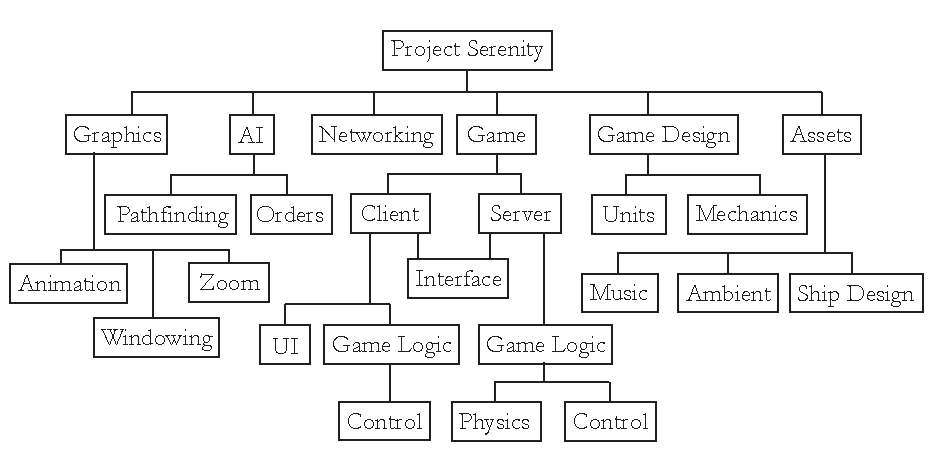
\includegraphics{res/wbs}
	\caption{Work Breakdown Structure of the game components}
\end{figure*}

From the WBS we can further break the project down into components which are suited for weekly development cycles.

Term 2 releases will include a UI, an AI system and further improvements to the components as required. Assets such as music and additional ship designs are non-essential and will likely follow in a later release.

\begin{figure}
	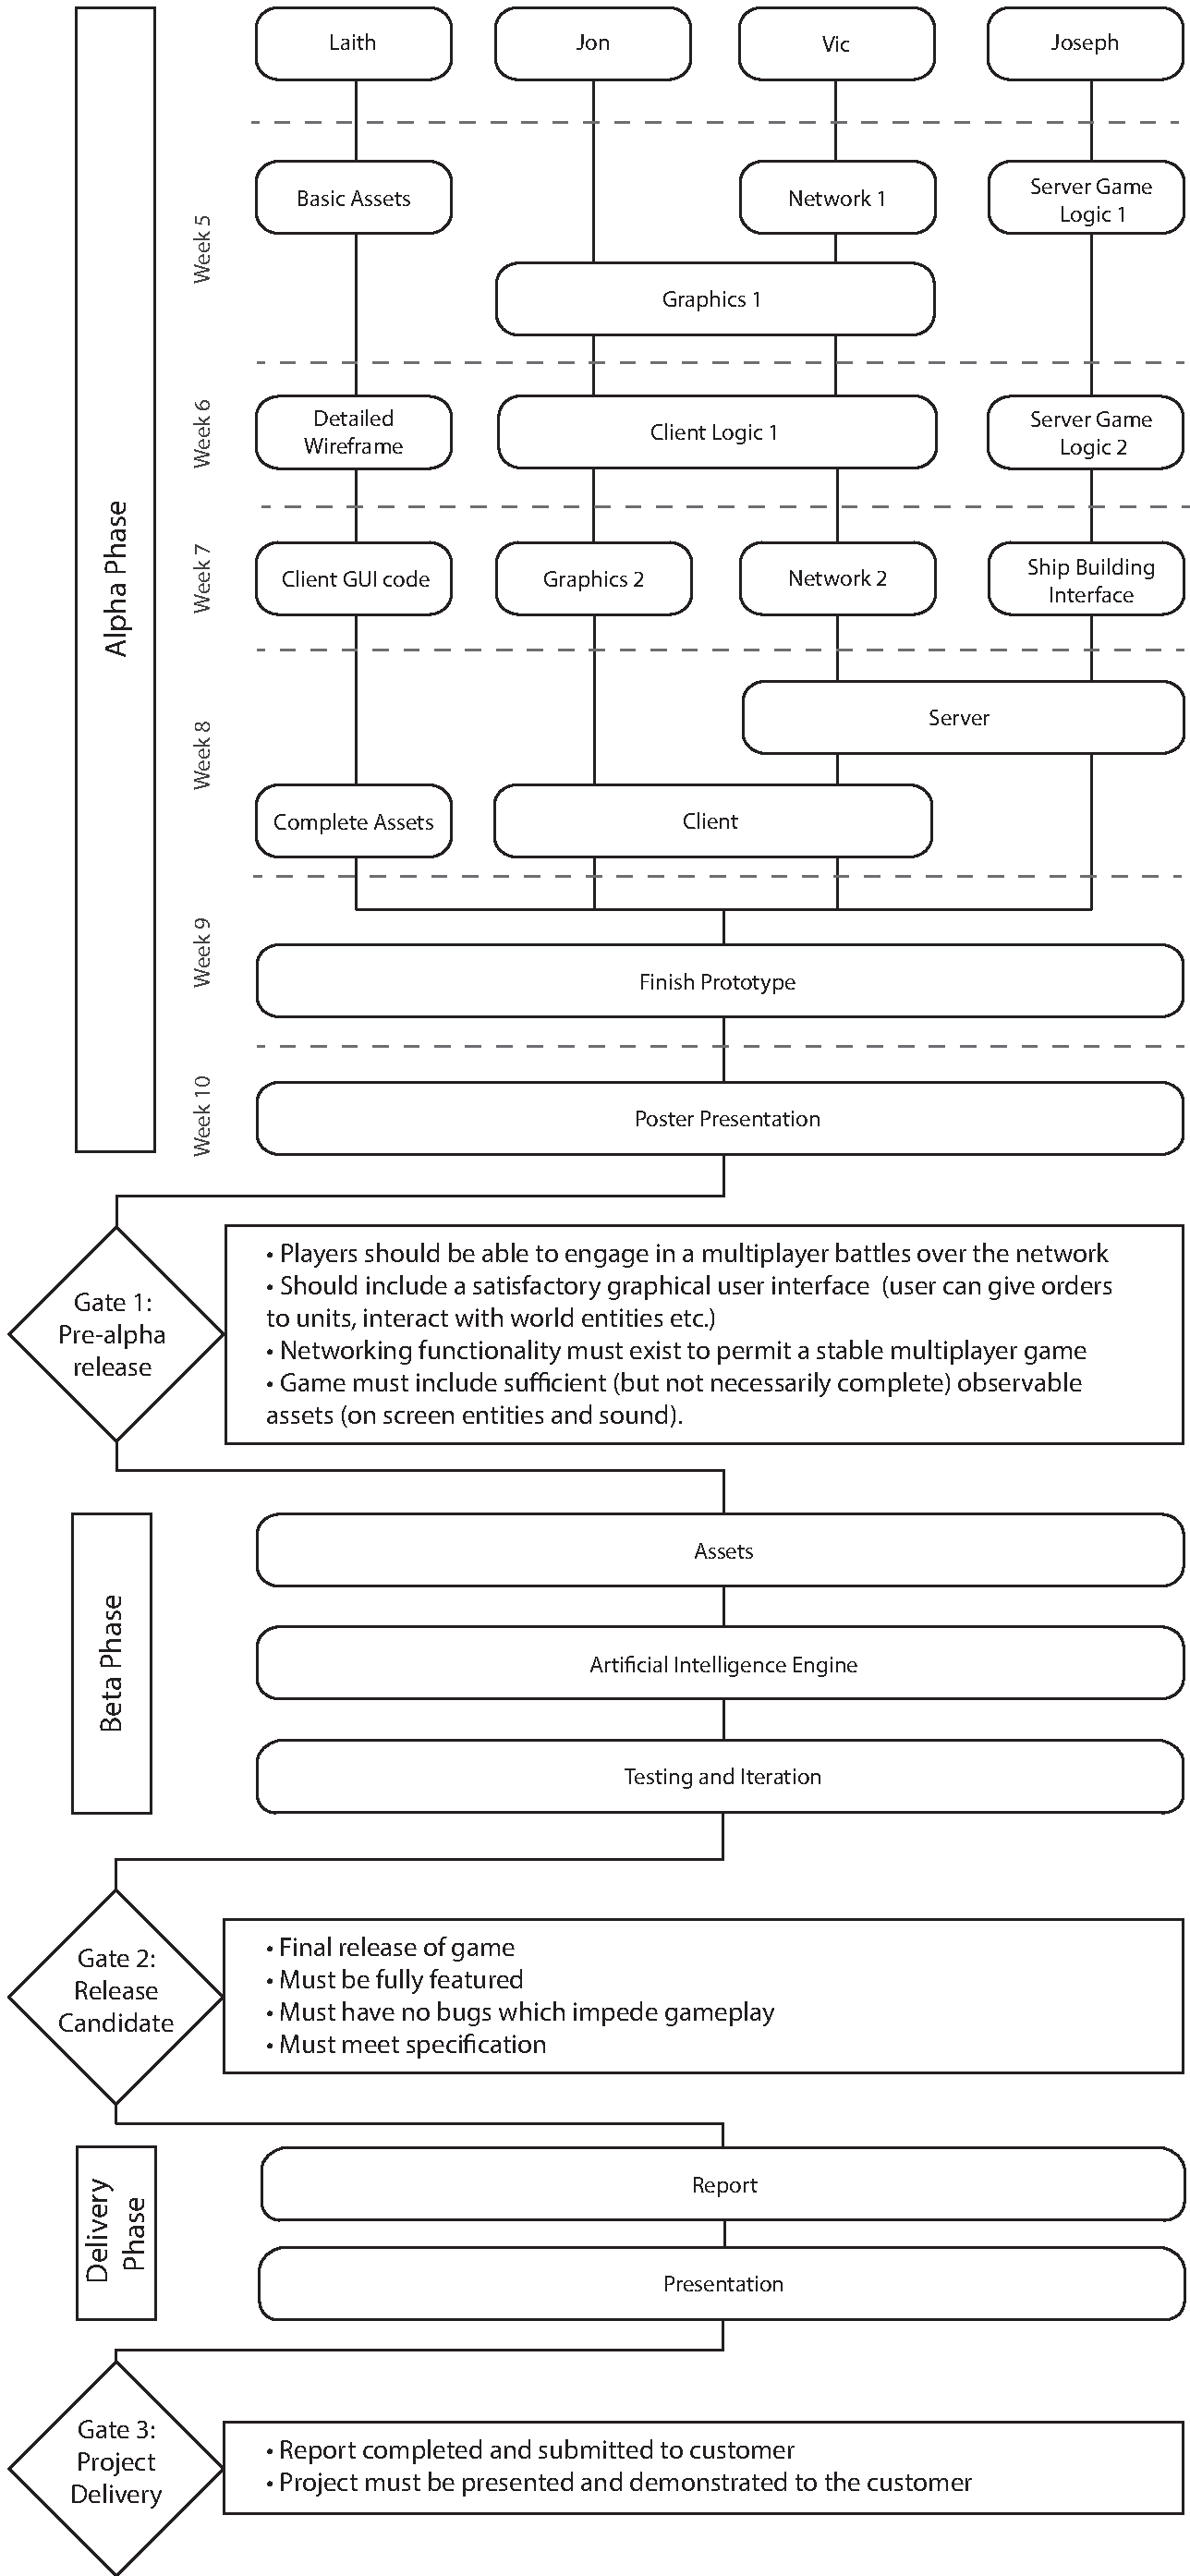
\includegraphics{res/stage_gate_diagram}
	% WE COULD PUT STANDARDS IN THE MARGIN!!! YES! CHEWING!!
	\caption{Stage-gate model of work breakdown structure showing the division of labour across the various project phases. 
	The alpha phase is more thoroughly planned so we are able to see a weekly breakdown of tasks in the near future. The gates are project milestones, each of which details the requirements for proceeding through that gate into the next phase.}
\end{figure}

\section{Legal, Ethical, and Social Issues}
\label{section:professional_issues}

% legal
One potential legal issue faced by this project is the use of third party software.
It must be ensured that any third party libraries included in the code are licensed
appropriately. This means only using software with a permissive license (e.g. Apache, BSD, or MIT licenses) and no proprietary software.

Game publishers such as Electronic Arts, and Lion Head, consider their games as intelligectual property, copywriting their games.
It is infeasable to check that all previous games published don't bear great similarities which would result in a court case.

% ethical


- gaming addiction
  - campaigns will be 5 battles long, allowing players an escape after 5 battles.

- dependency on whales (0.4\% of Zynga's customers account for 80\% of it's  1 billion profits.



% social issues
- language game in: english
- racism
- vialence




